%Translate this Latex book chapter to Spanish. Output in Latex format. Rearrange bullet points (\items) into full paragraphs. Make sure that sentences are connected in a more fluid way as they come. Elaborate on incomplete ideas where appropriate.

\section{Tareas de Etiquetado de Secuencias o Etiquetado}
\begin{itemize}
  \item El etiquetado de secuencias o etiquetado es una tarea en PNL que difiere de la clasificación de documentos.
  \item El objetivo es asignar etiquetas o etiquetas a una oración representada como una secuencia de tokens $x_1, x_2, \dots, x_n$.
  \item En particular, el objetivo del etiquetado de secuencias es asignar etiquetas a palabras, o más generalmente, asignar etiquetas discretas a elementos discretos en una secuencia \cite{jacobbook}.
  \item Ejemplos conocidos de esta tarea son el etiquetado de partes del discurso (POS) y el reconocimiento de entidades nombradas (NER).
\end{itemize}

\section{Etiquetado de Partes del Discurso}
\textcolor{green}{\textbf{ENTRADA:}}
Los beneficios aumentaron en Boeing Co., superando fácilmente las previsiones en Wall Street, cuando su CEO Alan Mulally anunció los resultados del primer trimestre.  \vspace{0.5cm}

\textcolor{green}{\textbf{SALIDA:}}
Los beneficios\textcolor{red}{/N} aumentaron\textcolor{red}{/V} en\textcolor{red}{/P} Boeing\textcolor{red}{/N} Co.\textcolor{red}{/N} ,\textcolor{red}{/,} superando\textcolor{red}{/V} fácilmente\textcolor{red}{/ADV} las\textcolor{red}{/DET} previsiones\textcolor{red}{/N} en\textcolor{red}{/P} Wall\textcolor{red}{/N} Street\textcolor{red}{/N} ,\textcolor{red}{/,} cuando\textcolor{red}{/P} su\textcolor{red}{/DET} CEO\textcolor{red}{/N} Alan\textcolor{red}{/N} Mulally\textcolor{red}{/N} anunció\textcolor{red}{/V} los\textcolor{red}{/DET} resultados\textcolor{red}{/N} del\textcolor{red}{/PREP} primer\textcolor{red}{/ADJ} trimestre\textcolor{red}{/N} .\textcolor{red}{/.}  \vspace{0.5cm}

\begin{itemize}
  \item \textcolor{red}{N} = \textcolor{blue}{Sustantivo}
  \item \textcolor{red}{V} = \textcolor{blue}{Verbo}
  \item \textcolor{red}{P} = \textcolor{blue}{Preposición}
  \item \textcolor{red}{Adv} = \textcolor{blue}{Adverbio}
  \item \textcolor{red}{Adj} = \textcolor{blue}{Adjetivo}
  \item ...
\end{itemize}

\begin{figure}[h]
  \includegraphics[scale=0.34]{pics/posTags.png}
\end{figure}
Fuente: \cite{JurafskyBook}

\section{Reconocimiento de Entidades Nombradas (NER)}
Una \textbf{entidad nombrada} es, hablando en términos generales, cualquier cosa a la que se puede hacer referencia con un nombre propio: una persona, un lugar, una organización. \vspace{0.5cm}

\textcolor{green}{\textbf{ENTRADA:}}
Los beneficios aumentaron en Boeing Co., superando fácilmente las previsiones en Wall Street, cuando su CEO Alan Mulally anunció los resultados del primer trimestre.  \vspace{0.5cm}

\textcolor{green}{\textbf{SALIDA:}}
Los beneficios aumentaron en \textcolor{red}{[Compañía} Boeing Co.\textcolor{red}{]}, superando fácilmente las previsiones en \textcolor{red}{[Lugar} Wall Street\textcolor{red}{]}, cuando su CEO \textcolor{red}{[Persona} Alan Mulally\textcolor{red}{]} anunció los resultados del primer trimestre. \vspace{0.5cm}

\begin{itemize}
  \item Dado que las entidades pueden abarcar varias palabras (es decir, un problema de reconocimiento de fragmentos), podemos utilizar el etiquetado BIO \cite{ramshaw1999text} para convertir el problema en un problema de etiquetado de secuencias.
  \item Etiquetado BIO: utilizar etiquetas que capturen tanto el límite como el tipo de entidad nombrada.
\end{itemize}

\paragraph{Etiquetado BIO: NER como Etiquetado de Secuencias}
\textcolor{green}{\textbf{ENTRADA:}}
Los beneficios aumentaron en Boeing Co., superando fácilmente las previsiones en Wall Street, cuando su CEO Alan Mulally anunció los resultados del primer trimestre.  \vspace{0.5cm}

\textcolor{green}{\textbf{SALIDA:}}
Los\textcolor{red}{/O} beneficios\textcolor{red}{/O} aumentaron\textcolor{red}{/O} en\textcolor{red}{/O} Boeing\textcolor{purple}{/B-C} Co.\textcolor{purple}{/I-C} ,\textcolor{red}{/O} superando\textcolor{red}{/O} fácilmente\textcolor{red}{/O} las\textcolor{red}{/O} previsiones\textcolor{red}{/O} en\textcolor{red}{/O} Wall\textcolor{purple}{/B-L} Street\textcolor{purple}{/I-L} ,\textcolor{red}{/O} cuando\textcolor{red}{/O} su\textcolor{red}{/O} CEO\textcolor{red}{/O} Alan\textcolor{purple}{/B-P} Mulally\textcolor{purple}{/I-P} anunció\textcolor{red}{/O} los\textcolor{red}{/O} resultados\textcolor{red}{/O} del\textcolor{red}{/O} primer\textcolor{red}{/O} trimestre\textcolor{red}{/O} .\textcolor{red}{/O}  \vspace{0.5cm}

\begin{itemize}
  \item \textcolor{red}{O} = \textcolor{blue}{Fuera (sin entidad)}
  \item \textcolor{purple}{B-C} = \textcolor{blue}{Comienzo de Compañía}
  \item \textcolor{purple}{I-C} = \textcolor{blue}{Dentro de Compañía}
  \item \textcolor{purple}{B-L} = \textcolor{blue}{Comienzo de Lugar}
  \item \textcolor{purple}{I-L} = \textcolor{blue}{Dentro de Lugar}
  \item \textcolor{purple}{B-P} = \textcolor{blue}{Comienzo de Persona}
  \item \textcolor{purple}{I-P} = \textcolor{blue}{Dentro de Persona}
\end{itemize}

Nuestro objetivo:
\textbf{Conjunto de entrenamiento:}
\begin{enumerate}
  \item Pierre\textcolor{red}{/NNP} Vinken\textcolor{red}{/NNP},\textcolor{red}{/,} 61\textcolor{red}{/CD} años\textcolor{red}{/NNS} de edad\textcolor{red}{/JJ},\textcolor{red}{/,} se unirá a la junta directiva como director no ejecutivo el 29 de noviembre.\textcolor{red}{/NNP}
  \item El Sr.\textcolor{red}{/NNP} Vinken\textcolor{red}{/NNP} es presidente\textcolor{red}{/NN} de Elsevier\textcolor{red}{/NNP} N.V.\textcolor{red}{/NNP}, el grupo editorial holandés.\textcolor{red}{/NNP}
  \item Rudolph\textcolor{red}{/NNP} Agnew\textcolor{red}{/NNP},\textcolor{red}{/,} de 55\textcolor{red}{/CD} años\textcolor{red}{/NNS} y presidente\textcolor{red}{/NN} de\ldots
\end{enumerate}

\subsection{Etiquetado de secuencias como aprendizaje supervisado}

\begin{itemize}
  \item Tenemos una secuencia de entradas $x = (x_1, x_2, \ldots, x_n)$ y las etiquetas correspondientes $y = (y_1, y_2, \ldots, y_n)$.
  \item La tarea consiste en aprender una función $f$ que mapea secuencias de entrada a secuencias de etiquetas: $f(x_1,x_2, \ldots, x_n) = y_1, y_2, \ldots, y_n$.
  \item Tenemos un conjunto de entrenamiento de secuencias etiquetadas: $\{(x^{(1)}, y^{(1)}), (x^{(2)}, y^{(2)}), \ldots, (x^{(m)}, y^{(m)})\}$.
\end{itemize}

\subsection{Enfoque generativo para el etiquetado de secuencias}

\begin{itemize}
  \item Los modelos generativos, como el clasificador de Naive Bayes utilizado para clasificación, también se pueden utilizar para tareas de etiquetado de secuencias en PLN.
  \item Enfoque:
  \begin{itemize}
    \item Entrenamiento: Aprender la distribución conjunta $p(x_1,x_2, \ldots, x_n,y_1, y_2, \ldots, y_n)$ de las secuencias de entrada.
    \item Decodificación: Utilizar la distribución aprendida para predecir secuencias de etiquetas para nuevas secuencias de entrada.
  \end{itemize}
  \item La decodificación en el etiquetado de secuencias implica encontrar la secuencia de etiquetas con la mayor probabilidad conjunta: $\arg\max_{y_1, y_2, \ldots, y_n}p(x_1,x_2, \ldots, x_n,y_1, y_2, \ldots, y_n)$.
\end{itemize}

\section{Modelos Ocultos de Markov}

\begin{itemize}
  \item Los Modelos Ocultos de Markov (HMM, por sus siglas en inglés) proporcionan una forma sistemática de manejar problemas de etiquetado de secuencias mediante modelos generativos y algoritmos de decodificación eficientes.
  \item Tenemos una oración de entrada $x = x_1, x_2, \ldots, x_n$ ($x_i$ es la $i$-ésima palabra en la oración).
  \item Tenemos una secuencia de etiquetas $y = y_1, y_2, \ldots, y_n$ ($y_i$ es la $i$-ésima etiqueta en la oración).
  \item Usaremos un HMM para definir $p(x_1, x_2, \ldots, x_n, y_1, y_2, \ldots, y_n)$ para cualquier oración $x_1, \ldots, x_n$ y secuencia de etiquetas $y_1, \ldots, y_n$ de la misma longitud \cite{kupiec1992robust}.
  \item Luego, la secuencia de etiquetas más probable para $x$ es:
  \[
    \arg\max_{y_1,\ldots, y_n} p(x_1, \ldots, x_n, y_1, \ldots, y_n)
  \]
\end{itemize}

\section{Modelos Ocultos de Markov Trigramas (Trigram HMM)}

Para cualquier oración $x_1, \ldots, x_n$ donde $x_i \in V$ para $i = 1, \ldots, n$, y cualquier secuencia de etiquetas $y_1, \ldots, y_{n+1}$ donde $y_i \in S$ para $i = 1, \ldots, n$, y $y_{n+1} = \text{STOP}$, la probabilidad conjunta de la oración y la secuencia de etiquetas es:
\[
  p(x_1, \ldots, x_n, y_1, \ldots, y_{n+1}) = \prod_{i=1}^{n+1} q(y_i | y_{i-2}, y_{i-1}) \prod_{i=1}^{n} e(x_i | y_i)
\]
donde hemos asumido que $x_0 = x_{-1} = *$.

\subsection{Parámetros del modelo}

\begin{itemize}
  \item $q(s|u, v)$ para cualquier $s \in S \cup \{\text{STOP}\}$, $u, v \in S \cup \{*\}$
  \begin{itemize}
    \item El valor de $q(s|u,v)$ se puede interpretar como la probabilidad de ver la etiqueta $s$ inmediatamente después del bigrama de etiquetas $(u, v)$.
  \end{itemize}
  \item $e(x|s)$ para cualquier $s \in S$, $x \in V$ 
  \begin{itemize}
    \item El valor de $e(x|s)$ se puede interpretar como la probabilidad de ver la observación $x$ emparejada con el estado $s$.
  \end{itemize}
\end{itemize}

\paragraph{Un ejemplo}

Si tenemos $n = 3$, $x_1, x_2, x_3$ igual a la oración ``the dog laughs'', y $y_1, y_2, y_3, y_4$ igual a la secuencia de etiquetas ``D N V STOP'', entonces:
\[
\begin{aligned}
p(x_1, \ldots, x_n, y_1, \ldots, y_{n+1}) = & q(D|*,*) \times q(N|*,D) \\
& \times q(V|D,N) \times q(\text{STOP}|N,V) \\
& \times e(\text{el}|D) \times e(\text{perro}|N) \times e(\text{se}|V) \times e(\text{ríe}|STOP)
\end{aligned}
\]
\begin{itemize}
  \item STOP es una etiqueta especial que termina la secuencia.
  \item Tomamos $y_0 = y_{-1} = *$, donde $*$ es un símbolo especial de "padding".
\end{itemize}

\section{Supuestos de independencia en los HMM trigramas}

\begin{itemize}
  \item Los Modelos Ocultos de Markov trigramas (HMM trigramas) se derivan

mediante la realización de supuestos específicos de independencia en el modelo.

  \item Consideremos dos secuencias de variables aleatorias: $X_1, \ldots, X_n$ y $Y_1, \ldots, Y_n$, donde $n$ es la longitud de las secuencias.

  \item Cada $X_i$ puede tomar cualquier valor en un conjunto finito $V$ de palabras, y cada $Y_i$ puede tomar cualquier valor en un conjunto finito $K$ de etiquetas posibles (por ejemplo, $K=\{D,N,V, \ldots \}$).

  \item Nuestro objetivo es modelar la probabilidad conjunta:

  \begin{align*}
    P(x_1,x_2,\dots,x_n,&y_1,\dots,y_n) \\
    &= p(y_1) \times p(y_2|y_1) \\
    &\quad \times \dots \\
    &\quad \times p(y_n|y_{n-1},y_{n-2},\dots y_1) \\
    &\quad \times p(x_1|y_{n},y_{n-1},\dots y_1) \\
    &\quad \times p(x_2|x_1,y_{n},y_{n-1},\dots y_1) \\
    &\quad \times p(x_n|x_{n-1},\dots,x_1,y_{n},y_{n-1},\dots y_1)
  \end{align*}

  \item Definimos una variable aleatoria adicional $Y_{n+1}$ que siempre toma el valor "STOP".

  \item La idea clave en los HMM es la factorización de la probabilidad conjunta:
  \[P(X_1 = x_1, \ldots, X_n = x_n, Y_1 = y_1, \ldots, Y_{n+1} = y_{n+1})\]
  \[= \prod_{i=1}^{n+1} P(Y_i = y_i | Y_{i-2} = y_{i-2}, Y_{i-1} = y_{i-1}) \times \prod_{i=1}^{n} P(X_i = x_i | Y_i = y_i)\]

  \item Primero asumimos que:
  \[P(Y_i = y_i | Y_{i-2} = y_{i-2}, Y_{i-1} = y_{i-1}) = q(y_i | y_{i-2}, y_{i-1})\]

  \item Esto asume que la secuencia $Y_1, \ldots, Y_{n+1}$ es una secuencia de Markov de segundo orden, donde cada estado depende solo de los dos estados anteriores.

  \item Y también asumimos que:
    \[P(X_i = x_i | Y_i = y_i) = e(x_i | y_i)\]

  \item Esto asume que las observaciones y los estados están condicionalmente independientes dadas las etiquetas.

\end{itemize}


\section{¿Por qué el nombre?}
\[
\begin{aligned}
  p(x_1, \ldots, x_n, y_1, \ldots, y_n) = & q(\text{STOP}|y_{n-1}, y_n) \\
  & \times \prod_{j=1}^{n} q(y_j | y_{j-2}, y_{j-1}) \\
  & \times \prod_{j=1}^{n} e(x_j | y_j)
\end{aligned}
\]
Los componentes de la cadena de Markov:
\[
q(\text{STOP}|y_{n-1}, y_n)\times \prod_{j=1}^{n} q(y_j | y_{j-2}, y_{j-1})
\]
Estas transiciones no se observan directamente para una secuencia dada de palabras $(x_1, \ldots, x_n)$, de ahí el nombre de "ocultas".

El componente observable:
\[
\prod_{j=1}^{n} e(x_j | y_j)
\]
El componente observable de los HMM modela las probabilidades de emisión de los símbolos observados ($x$) condicionados a los estados ocultos correspondientes ($y$).

\section{Estimación Suavizada}

\[
\begin{aligned}
q(Vt | DT, JJ) = & \lambda_1 \times \frac{{\text{Count}(Dt, JJ, Vt)}}{{\text{Count}(Dt, JJ)}} \\
& + \lambda_2 \times \frac{{\text{Count}(JJ, Vt)}}{{\text{Count}(JJ)}} \\
& + \lambda_3 \times \frac{{\text{Count}(Vt)}}{{\text{Count}()}}
\end{aligned}
\]

donde $\lambda_1 + \lambda_2 + \lambda_3 = 1$, y para todo $i$, $\lambda_i \geq 0$.

\vspace{0.5cm}

\[
e(\text{base} | Vt) = \frac{{\text{Count}(Vt, \text{base})}}{{\text{Count}(Vt)}}
\]

\section{Tratando con Palabras de Baja Frecuencia}

Un método común es el siguiente:
\begin{itemize}
  \item Paso 1: Dividir el vocabulario en dos conjuntos
    \begin{itemize}
      \item Palabras frecuentes = palabras que ocurren $\geq 5$ veces en el entrenamiento
      \item Palabras de baja frecuencia = todas las demás palabras
    \end{itemize}
  \item Paso 2: Mapear las palabras de baja frecuencia a un conjunto pequeño y finito, dependiendo de prefijos, sufijos, etc.
\end{itemize}

A continuación se muestra un ejemplo de clases de palabras para el reconocimiento de entidades nombradas \cite{bikelSW99}:

\[
\begin{array}{l|l|l}
  \text{Clase de palabra} & \text{Ejemplo}  & \text{Intuición} \\
  \hline
  \text{twoDigitNum} & 90 & \text{Año de dos dígitos} \\
  \text{fourDigitNum} & 1990 & \text{Año de cuatro dígitos} \\
  \text{containsdígito y letra} & A8956-67 & \text{Código de producto} \\
  \text{containsDigitAndDash} & 09-96 & \text{Fecha} \\
  \text{containsDigitAndSlash} & 11/9/89 & \text{Fecha} \\
  \text{containsDigitAndComma} & 23,000.00 & \text{Cantidad monetaria} \\
  \text{containsDigitAndPeriod} & 1.00 & \text{Cantidad monetaria, porcentaje} \\
  \text{othernum} & 456789 & \text{Otro número} \\
  \text{allCaps} & BBN & \text{Organización} \\
  \text{capPeriod} & M. & \text{Inicial de nombre de persona} \\
  \text{firstWord} & \text{Primera palabra de la oración} & \text{Sin información útil de capitalización} \\
  \text{initCap} & \text{Sally} & \text{Palabra capitalizada} \\
  \text{lowercase} & \text{can} & \text{Palabra sin capitalizar} \\
  \text{other} & , & \text{Signos de puntuación, todas las demás palabras} \\
\end{array}
\]



\section{Problema de Decodificación}
Problema de decodificación: Para una entrada $x_1 \ldots x_n$, encontrar
\[
\arg \max_{y_1 \ldots y_{n+1}} p(x_1 \ldots x_n, y_1 \ldots y_{n+1})
\]
donde $\arg \max$ se toma sobre todas las secuencias $y_1 \ldots y_{n+1}$ tales que $y_i \in S$ para $i = 1 \ldots n$, y $y_{n+1} = \text{STOP}$.

Suponemos que $p$ toma la forma:
\[
p(x_1 \ldots x_n, y_1 \ldots y_{n+1}) = \prod_{i=1}^{n+1} q(y_i|y_{i-2}, y_{i-1}) \prod_{i=1}^{n} e(x_i|y_i)
\]

Recordemos que hemos asumido en esta definición que $y_0 = y_{-1} = *$ y $y_{n+1} =$ STOP.

\subsection{Método Bruto Ingenuo}

El método bruto ingenuo para encontrar la secuencia de etiquetas con la puntuación más alta es enumerar todas las posibles secuencias de etiquetas $y_1, \ldots, y_{n+1}$, calcular su puntuación utilizando la función $p$ y seleccionar la secuencia con la puntuación más alta.

\begin{itemize}
    \item Ejemplo:
    \begin{itemize}
        \item Oración de entrada: \textit{the dog barks}
        \item Conjunto de etiquetas posibles: $K = \{D, N, V\}$
    \end{itemize}
    
    \item Enumerar todas las posibles secuencias de etiquetas:
    \begin{itemize}
        \item $D\ D\ D\ STOP$
        \item $D\ D\ N\ STOP$
        \item $D\ D\ V\ STOP$
        \item $D\ N\ D\ STOP$
        \item $D\ N\ N\ STOP$
        \item $D\ N\ V\ STOP$
        \item ...
    \end{itemize}
\end{itemize} 
  
 En este caso, hay $3^3 = 27$ secuencias posibles. Sin embargo, para oraciones más largas, este método se vuelve ineficiente.Para una oración de entrada de longitud $n$, hay $|K|^n$ secuencias posibles de etiquetas. El crecimiento exponencial hace que la búsqueda exhaustiva sea impracticable para oraciones de longitud razonable.

\section{Decodificación de Viterbi con Programación Dinámica}

El algoritmo utilizado por los HMM para realizar una decodificación eficiente se denomina decodificación de Viterbi. La decodificación de Viterbi utiliza programación dinámica, que es una técnica para resolver problemas de optimización dividiéndolos en subproblemas superpuestos. Al almacenar las soluciones a estos subproblemas en una tabla, no es necesario recalcularlos, lo que mejora considerablemente la eficiencia de los algoritmos. A continuación, mostramos cómo funciona la programación dinámica con dos ejemplos: el factorial y Fibonacci.

\paragraph{Factorial}

\begin{itemize}
    \item Implementación recursiva:
    
    \begin{lstlisting}[language=Python]
def recur_factorial(n):
    # Caso base
    if n == 1:
        return n
    else:
        return n * recur_factorial(n-1)
    \end{lstlisting}
    
    \item Implementación con programación dinámica:
    
    \begin{lstlisting}[language=Python]
def dynamic_factorial(n):
    tabla = [0 for i in range(0, n+1)]
    
    # Caso base
    tabla[0] = 1
    
    for i in range(1, len(tabla)):
        tabla[i] = i * tabla[i-1]
    
    return tabla[n]
    \end{lstlisting}
\end{itemize}

\paragraph{Fibonacci}

\begin{itemize}
    \item Implementación recursiva:
    
    \begin{lstlisting}[language=Python]
def recur_fibonacci(n):
    if n == 1 or n == 0:
        return 1
    else:
        return recur_fibonacci(n-1) + recur_fibonacci(n-2)
    \end{lstlisting}
    
    \item Implementación con programación dinámica:
    
    \begin{lstlisting}[language=Python]
def dynamic_fibonacci(n):
    tabla = [0 for i in range(0, n+1)]
    
    # Caso base
    tabla[0] = 1
    tabla[1] = 1
    
    for i in range(2, len(tabla)):
        tabla[i] = tabla[i-1] + tabla[i-2]
    
    return tabla[n]
    \end{lstlisting}
\end{itemize}

\paragraph{Complejidad}

En las implementaciones recursivas, la complejidad puede ser bastante alta debido a los cálculos repetidos de los mismos subproblemas. Sin embargo, la programación dinámica puede reducir significativamente la complejidad al almacenar las soluciones a los subproblemas en una tabla o matriz y reutilizarlas cuando sea necesario. Este enfoque elimina los cálculos redundantes y permite una computación más eficiente. En el caso de Fibonacci, la complejidad se reduce de exponencial a lineal.

\section{El Algoritmo de Viterbi}

El algoritmo de Viterbi calcula eficientemente la máxima probabilidad de una secuencia de etiquetas utilizando programación dinámica.

\textbf{Definiciones:}

\begin{itemize}
    \item Definimos $n$ como la longitud de la oración.
    \item Definimos $S_k$ para $k = -1 \ldots n$ como el conjunto de etiquetas pos

ibles en la posición $k$: $S_{-1} = S_0 = \{*\}$, $S_k = S$ para $k \in \{1 \ldots n\}$.
    \item Definimos una versión truncada de la probabilidad codificada por el HMM hasta la posición $k$, $r(y_{-1}, y_0, y_1, \ldots, y_k)$, como:
    
    \[
    r(y_{-1}, y_0, y_1, \ldots, y_k) = \prod_{i=1}^{k} q(y_i | y_{i-2}, y_{i-1})
    \]
    
    \item Definimos una tabla de programación dinámica $\pi(k, u, v)$ como la máxima probabilidad de una secuencia de etiquetas que termina en las etiquetas $u, v$ en la posición $k$:
    
    \[
    \pi(k, u, v) = \max_{y_{-1}, y_0, y_1, \ldots, y_k : y_{k-1} = u, y_k = v} r(y_{-1}, y_0, y_1, \ldots, y_k)
    \]
\end{itemize}

\paragraph{Un Ejemplo}

Recuerde que $\pi(k, u, v)$ es la máxima probabilidad de una secuencia de etiquetas que termina en las etiquetas $u, v$ en la posición $k$.

\begin{figure}[h]
    \centering
    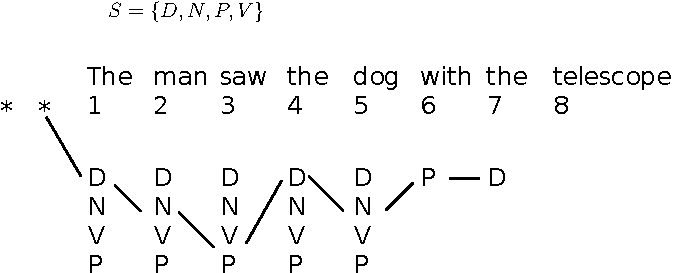
\includegraphics[scale = 0.6]{pics/viterbi1.pdf}
\end{figure}

\begin{itemize}
    \item Hay muchas secuencias posibles de etiquetas.
    \item Cada una de ellas tiene una probabilidad calculada a partir de los parámetros $q$ y $e$.
    \item $\pi(7, P, D)$ es la máxima probabilidad de que una de estas secuencias de etiquetas termine en $P$ y $D$ en la posición $7$.
    \item La ruta representa la secuencia con la máxima probabilidad.
\end{itemize}

\subsection{Una Definición Recursiva}

\textbf{Caso base:}

\[
\pi(0, *, *) = 1
\]

\textbf{Definición recursiva:}

Para cualquier $k \in \{1 \ldots n\}$, para cualquier $u \in S_{k-1}$ y $v \in S_k$:

\[
\pi(k, u, v) = \max_{w \in S_{k-2}} (\pi(k - 1, w, u) \times q(v|w, u) \times e(x_k|v))
\]

\paragraph{Justificación de la Definición Recursiva}

Para cualquier $k \in \{1 \ldots n\}$, para cualquier $u \in S_{k-1}$ y $v \in S_k$:

\[
\pi(k, u, v) = \max_{w \in S_{k-2}} (\pi(k - 1, w, u) \times q(v|w, u) \times e(x_k|v))
\]

\begin{figure}[h]
    \centering
    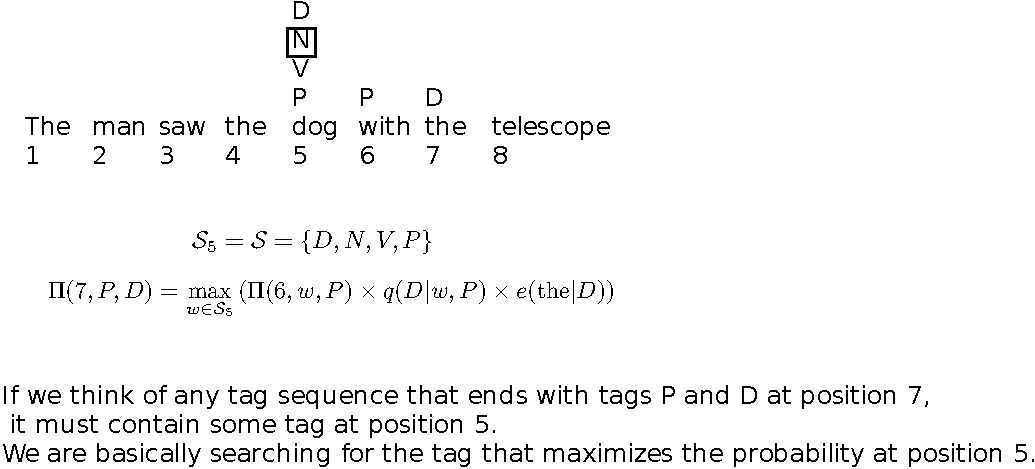
\includegraphics[scale = 0.6]{pics/viterbi2.pdf}
\end{figure}



\begin{itemize}
    \item Consideremos una secuencia de etiquetas arbitraria que termina con las etiquetas $P$ y $D$ en la posición $7$.
    \item Debe contener alguna etiqueta en la posición $5$.
    \item Básicamente, estamos buscando la etiqueta que maximiza la probabilidad en la posición $5$.
\end{itemize}

\subsection{El Algoritmo de Viterbi}

\begin{algorithm}[H]
\SetKwInput{Input}{Entrada}
\SetKwInput{Initialization}{Inicialización}
\SetKwFunction{Max}{max}
\SetKwFunction{Return}{retornar}

\Input{una oración $x_1 \ldots x_n$, parámetros $q(s|u, v)$ y $e(x|s)$}

\Initialization{Establecer $\pi(0, *, *) = 1$;  $S_{-1} = S_0 = \{*\}$, $S_k = S$ para $k \in \{1 \ldots n\}$.
}

\BlankLine
\SetAlgoLined
\caption{Algoritmo de Viterbi}
\label{algo:prob_inference}
\BlankLine

\For{$k = 1$ \KwTo $n$}{
\For{$u \in S_{k-1}, v \in S_k$}{
$\pi(k, u, v) = \max_{w \in S_{k-2}} (\pi(k - 1, w, u) \times q(v|w, u) \times e(x_k|v))$
}
}

\BlankLine
\Return{$\max_{u \in S_{n-1}, v \in S_n} (\pi(n, u, v) \times q(\text{STOP}|u, v))$}
\end{algorithm}

\subsection{El Algoritmo de Viterbi con Punteros de Retroceso}

\begin{algorithm}[H]
\SetKwInput{Input}{Entrada}
\SetKwInput{Initialization}{Inicialización}
\SetKwFunction{Max}{max}
\SetKwFunction{ArgMax}{argmax}
\SetKwFunction{Return}{retornar}

\Input{una oración $x_1 \ldots x_n$, parámetros $q(s|u, v)$ y $e(x|s)$}

\Initialization{Establecer $\pi(0, *, *) = 1$;  $S_{-1} = S_0 = \{*\}$, $S_k = S$ para $k \in \{1 \ldots n\}$.
}

\BlankLine
\SetAlgoLined
\caption{Algoritmo de Viterbi con Punteros de Retroceso}
\label{algo:viterbi}
\BlankLine

\For{$k = 1$ \KwTo $n$}{
\For{$u \in S_{k-1}, v \in S_k$}{
\[
\pi(k, u, v) = \max_{w \in S_{k-2}} (\pi(k - 1, w, u) \times q(v|w, u) \times e(x_k|v))
\]    
\[
\text{bp}(k, u, v) = \arg \max_{w \in S_{k-2}} (\pi(k - 1, w, u) \times q(v|w, u) \times e(x_k|v))
    \]} 
}



\BlankLine
$(y_{n-1}, y_n) = \arg \max_{(u,v)} (\pi(n, u, v) \times q(\text{STOP}|u, v))$ \tcp*[r]{Find maximum probability and corresponding tags}
\For{$k = (n - 2)$ \KwTo $1$}{
$y_k = \text{bp}(k + 2, y_{k+1}, y_{k+2})$ \tcp*[r]{Retrieve tag sequence using backpointers}
}

\BlankLine
\Return{the tag sequence $y_1 \ldots y_n$} \tcp*[r]{Return the final tag sequence}
\end{algorithm}

En el Algoritmo \ref{algo:viterbi}, se utiliza el puntero de retroceso para reconstruir la secuencia de etiquetas con la máxima probabilidad. El algoritmo recorre las tablas $\pi$ en orden inverso, comenzando desde la posición $n$ hasta la posición $1$. En cada iteración, se elige la etiqueta $u$ y $v$ que maximizan la expresión $\pi(k, u, v) \times q(\text{STOP}|u, v)$. Estas etiquetas se agregan al comienzo de la secuencia de etiquetas $path$, y al final del algoritmo, se devuelve la secuencia $path[1:-1]$, eliminando las etiquetas de inicio y detención.

Con el algoritmo de Viterbi, podemos encontrar eficientemente la secuencia de etiquetas más probable para una oración dada, utilizando programación dinámica y aprovechando la estructura de dependencia entre las etiquetas en el HMM. Esto es especialmente útil en problemas de etiquetado de secuencias, como el etiquetado de partes del habla en NLP. 

\subsection{El Algoritmo de Viterbi: Tiempo de Ejecución}
El tiempo de ejecución del algoritmo de Viterbi se puede analizar de la siguiente manera:

\begin{itemize}
    \item Se requiere un tiempo de $O(n|S|^3)$ para calcular $q(s|u, v) \times e(x_k|s)$ para todos los valores de $k, s, u, v$.
    \item La tabla $\pi$ tiene $n|S|^2$ entradas que deben ser llenadas.
    \item Se necesita un tiempo de $O(|S|)$ para llenar una entrada.
\end{itemize}

Por lo tanto, el tiempo de ejecución total es $O(n|S|^3)$.

\paragraph{Ventajas y Desventajas}
El uso de etiquetadores basados en Modelos de Markov Ocultos (HMM) presenta ciertas ventajas y desventajas:

\begin{itemize}
    \item Los etiquetadores HMM son fáciles de entrenar (se recopilan conteos a partir de un corpus de entrenamiento).
    \item Tienen un rendimiento relativamente bueno (más del 90\% de precisión en el reconocimiento de entidades nombradas).
    \item La principal dificultad radica en modelar $e(\text{palabra} | \text{etiqueta})$, lo cual puede ser muy complejo si las "palabras" son complejas.
\end{itemize}

Aunque los etiquetadores HMM tienen ventajas en términos de simplicidad y rendimiento, la modelización de la probabilidad condicional $e(\text{palabra} | \text{etiqueta})$ puede resultar desafiante en situaciones donde las palabras son complejas o ambiguas. En tales casos, se pueden requerir técnicas más avanzadas para mejorar la precisión del etiquetado de secuencias.


\section{MEMMs}

\begin{itemize}

\item Los modelos de Markov de entropía máxima (MEMMs) utilizan modelos log-lineales multiclase para tareas de etiquetado de secuencias \cite{mccallum2000maximum}.

\item En la literatura temprana de PLN, la regresión logística a menudo se llamaba clasificación de entropía máxima \cite{jacobbook}.

\item Por lo tanto, los MEMMs se parecerán mucho a los modelos de softmax multiclase vistos en la conferencia sobre modelos lineales.

\item A diferencia de los HMM, aquí confiamos en funciones parametrizadas.

\item El objetivo de los MEMMs es modelar la siguiente distribución condicional:

\begin{displaymath}
P(s_1,s_2 \dots, s_m | x_1, \dots, x_m)
\end{displaymath}

\item Donde cada $x_j$ para $j = 1 \dots m$ es el símbolo de entrada $j$ (por ejemplo, la $j$-ésima palabra en una oración), y cada $s_j$ para $j = 1 \dots m$ es la $j$-ésima etiqueta\footnote{Estas diapositivas se basan en notas de conferencia de Michael Collins \url{http://www.cs.columbia.edu/~mcollins/crf.pdf}. La notación y la terminología se han adaptado para ser coherentes con el resto del curso.}.

\item Esperaríamos que $P$(DET, NOUN, VERB$|$the, dog, barks$)$ sea mayor que $P$(VERB, VERB, VERB$|$the, dog, barks$)$ en un modelo entrenado a partir de un conjunto de datos de entrenamiento de etiquetado POS.

\item Usamos $S$ para denotar el conjunto de etiquetas posibles.

\item Suponemos que $S$ es un conjunto finito.

\item Por ejemplo, en el etiquetado de partes del habla en inglés, $S$ sería el conjunto de todas las posibles partes del habla en inglés (sustantivo, verbo, determinante, preposición, etc.).

\item Dada una secuencia de palabras $x_1, \dots, x_m$, hay $k^m$ secuencias posibles de partes del habla $s_1, \dots, s_m$, donde $k = |S|$ es el número de partes del habla posibles.

\item Queremos estimar una distribución sobre estas $k^m$ secuencias posibles.

\item En un primer paso, los MEMMs usan la siguiente descomposición ($s_0$ siempre tiene una etiqueta especial $*$):

\begin{equation}
\begin{split}
P(s_1,s_2 \dots, s_m | x_1, \dots, x_m) \quad & = \prod_{i=1}^{m}    P(s_i | s_1 \dots, s_{i-1}, x_1, \dots, x_m)\\
\quad & = \prod_{i=1}^{m}    P(s_i | s_{i-1}, x_1, \dots, x_m)
\end{split}
\end{equation}

\item La primera igualdad es exacta (se sigue de la regla de la cadena de probabilidades condicionales).

\item La segunda igualdad se deriva de un supuesto de independencia, a saber, que para todo $i$,

\begin{displaymath}
P(s_i | s_1 \dots, s_{i-1}, x_1, \dots, x_m) = P(s_i | s_{i-1}, x_1, \dots, x_m)
\end{displaymath}

\item Por lo tanto, estamos haciendo una suposición de Markov de primer orden similar a la suposición de Markov realizada en los HMM\footnote{De hecho, hicimos una suposición de Markov de segundo orden en los HMM. Los MEMMs también se pueden extender a suposiciones de segundo orden.}.

\item La etiqueta en la posición $i$ depende solo de la etiqueta en la posición $(i-1)$.

\item Habiendo hecho estas suposiciones de independencia, luego modelamos cada término usando un modelo log-lineal multiclase (softmax):

\begin{equation}
P(s_i | s_{i-1}, x_1, \dots, x_m) = \frac{\exp (\vec{w}\cdot \vec{\phi}(x_1, \cdots, x_m, i, s_{i-1},s_i))}{\sum_{s' \in S} \exp (\vec{w}\cdot \vec{\phi}(x_1, \cdots, x_m, i, s_{i-1},s'))}
\end{equation}

\end{itemize}

Aquí, $\vec{\phi}(x_1, \cdots, x_m, i, s_{i-1},s_i)$ es un vector de características donde:
\begin{itemize}
\item $x_1, \cdots, x_m$ es la oración completa que se está etiquetando.
\item $i$ es la posición a etiquetar (puede tomar cualquier valor de $1$ a $m$).
\item $s_{i-1}$ es el valor de la etiqueta anterior (puede tomar cualquier valor en $S$).
\item $s_i$ es el nuevo valor de la etiqueta (puede tomar cualquier valor en $S$).

\end{itemize}

El alcance del vector de características está \textbf{restringido} a toda la secuencia de entrada $x_1, x_m$, y solo las etiquetas anteriores y actuales. Esta restricción permite el entrenamiento eficiente tanto de los MEMMs como de los CRFs.


\section{Ejemplo de características utilizadas en el etiquetado de partes del habla}

\begin{enumerate}
\item $\vec{\phi}(x_1, \cdots, x_m, i, s_{i-1},s_i)_{[1]}=1$ si $s_i$ = ADVERB y la palabra $x_i$ termina en ``-ly''; 0 en caso contrario. \\
Si el peso $\vec{w}_{[1]}$ asociado con esta característica es grande y positivo, entonces esta característica está diciendo básicamente que preferimos etiquetas donde las palabras que terminan en -ly se etiquetan como ADVERB.

\item $\vec{\phi}(x_1, \cdots, x_m, i, s_{i-1},s_i)_{[2]}=1$ si $i=1$, $s_i$=VERB y $x_m$= $?; 0$ en caso contrario. \\
Si el peso $\vec{w}_{[2]}$ asociado con esta característica es grande y positivo, entonces se prefieren las etiquetas que asignan VERB a la primera palabra de una pregunta (por ejemplo, "¿Es esta una oración que comienza con un verbo?").

\item $\vec{\phi}(x_1, \cdots, x_m, i, s_{i-1},s_i)_{[3]}=1$ si $s_{i-1}$=ADJECTIVE y $s_i$=NOUN; 0 en caso contrario. \\
Nuevamente, un peso positivo para esta característica significa que los adjetivos tienden a ir seguidos de sustantivos.

\item $\vec{\phi}(x_1, \cdots, x_m, i, s_{i-1},s_i)_{[4]}=1$ si $s_{i-1}$=PREPOSITION y $s_{i}$=PREPOSITION. \\
Un peso negativo $\vec{w}_{[4]}$ para esta función significaría que las preposiciones no tienden a seguir a las preposiciones.

\end{enumerate}

\footnotemark{Fuente: \url{https://blog.echen.me/2012/01/03/introduction-to-conditional-random-fields/}}



\section{Plantillas de características}

Es posible definir plantillas de características más generales que cubran unigramas, bigramas, n-gramas de palabras, así como valores de etiqueta de $s_{i-1}$ y $s_i$.

\begin{enumerate}

\item Una plantilla de características de unigramas de palabras y unigramas de etiquetas: $\vec{\phi}(x_1, \cdots, x_m, i, s_{i-1},s_i)_{[index(j,z)]}=1$ si $s_i$ = TAG$_{[j]}$ y $x_i$ = WORD$_{[z]}$; 0 en caso contrario $\forall j,z$. \\
Nótese que $j$ es un índice que abarca todas las etiquetas posibles en $S$ y $z$ es otro índice que abarca las palabras en el vocabulario $V$.

\item Una plantilla de características de bigramas de palabras y bigramas de etiquetas: $\vec{\phi}(x_1, \cdots, x_m, i, s_{i-1},s_i)_{[index(j,z,u,v)]}=1$ si $s_{i-1}$ = TAG$_{[j]}$, $s_i$ = TAG$_{[z]}$, $x_{i-1}$ = WORD$_{[u]}$ y $x_{i}$ = WORD$_{[v]}$; 0 en caso contrario $\forall j,z,u,v$.

\end{enumerate}

La función $index(j,k,...)$ asignará a cada característica diferente un índice único en el vector de características. \\
Nótese que el vector resultante tendrá una dimensión muy alta y será disperso.

\paragraph{Ejemplo}
\begin{figure}[h]
\caption{Ejemplo de características en el etiquetado de partes del habla}
\centering
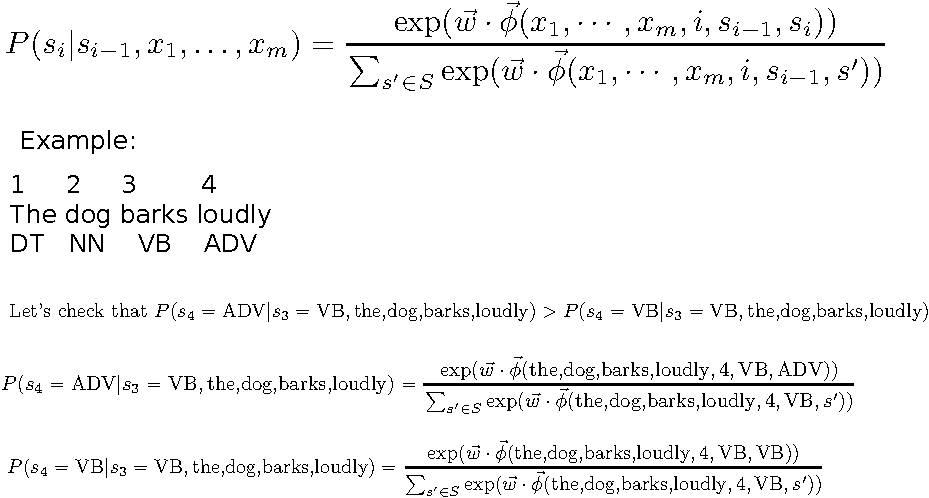
\includegraphics[scale = 0.73]{pics/CRF1.pdf}
\end{figure}

\begin{figure}[h]
\caption{Ejemplo de características en el etiquetado de partes del habla (continuación)}
\centering
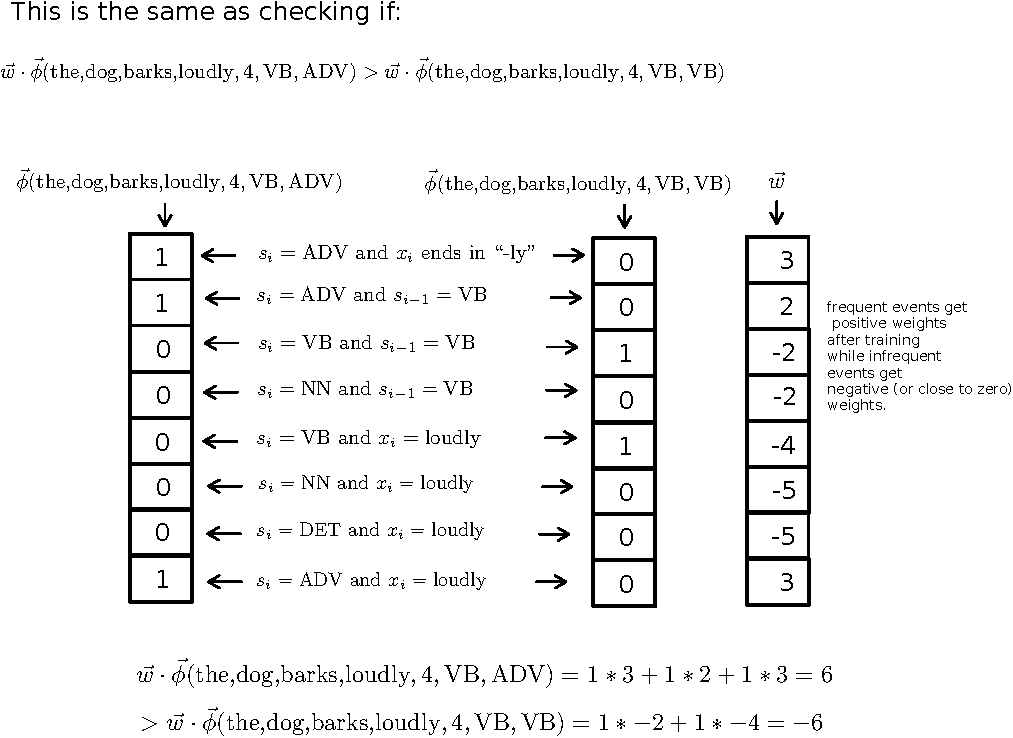
\includegraphics[scale = 0.6]{pics/CRF2.pdf}
\end{figure}

\section{MEMMs y Softmax Multiclase}

\begin{itemize}
\item Observemos que el modelo log-lineal mencionado anteriormente es muy similar al modelo softmax multiclase presentado en la conferencia sobre modelos lineales.

\item Un modelo log-lineal general tiene la siguiente forma:

\begin{displaymath}
P(y | x; \vec{w}) = \frac{\exp (\vec{w}\cdot \vec{\phi}(x,y))}{\sum_{y' \in Y} \exp (\vec{w}\cdot \vec{\phi}(x,y'))}
\end{displaymath}


\item Un modelo softmax multiclase tiene la siguiente forma:
\begin{equation}
\begin{split}
\hat{\vec{y}} \quad & =  \operatorname{softmax}(\vec{x} \cdot W + \vec{b})  \\
\hat{\vec{y}}_{[i]} \quad & = \frac{e^{(\vec{x} \cdot W + \vec{b})_{[i]}}}{\sum_j e^{(\vec{x} \cdot W + \vec{b})_{[j]}}}
\end{split}
\end{equation}


\item Diferencia 1: en el modelo log-lineal tenemos un vector de parámetros fijo $\vec{w}$ en lugar de tener múltiples vectores (una columna de $W$ por cada valor de clase).

\item Diferencia 2: el vector de características del modelo log-lineal $\vec{\phi}(x,y)$ incluye información de la etiqueta $y$, mientras que el vector de entrada $\vec{x}$ del modelo softmax es independiente de $y$.

\item Los modelos log-lineales permiten usar características que consideran la interacción entre $x$ e $y$ (por ejemplo, $x$ termina en ``ly'' e $y$ es un ADVERBIO).


\end{itemize}



\section{Entrenamiento de los MEMMs}

\begin{itemize}

\item Una vez que hemos definido los vectores de características $\vec{\phi}$, podemos entrenar los parámetros $\vec{w}$ del modelo de la misma manera que se entrenan los modelos lineales.

\item Establecemos la log-verosimilitud negativa como función de pérdida y optimizamos los parámetros utilizando descenso de gradiente a partir de los ejemplos de entrenamiento.

\item Esto es equivalente a usar la pérdida de entropía cruzada.

\item "Cualquier pérdida que consista en una log-verosimilitud negativa es una entropía cruzada entre la distribución empírica definida por el conjunto de entrenamiento y la distribución de probabilidad definida por el modelo" \cite{goodfellow2016deep}.

\end{itemize}


\section{Decodificación con MEMMs}

\begin{itemize}

\item El problema de decodificación es el siguiente.

\item Se nos proporciona una nueva secuencia de prueba $x_1, \dots, x_m$.

\item Nuestro objetivo es calcular la secuencia de estados más probable para esta secuencia de prueba,

\begin{equation}
\operatorname{arg} \max_{s_1,\dots,s_m} P(s_1,\dots,s_m|x_1,\dots,x_m).
\end{equation}

\item Hay $k^m$ posibles secuencias de estados, por lo que para cualquier longitud de oración razonablemente grande $m$, la búsqueda exhaustiva de todas las posibilidades no será posible.

\item Podemos usar el algoritmo de Viterbi de manera similar a como se usa para los HMM.

\item La estructura de datos básica en el algoritmo será una tabla de programación dinámica $\pi$ con entradas $\pi[j,s]$ para $j=1, \dots, m$ y $s \in S$.

\item $\pi[j,s]$ almacenará la probabilidad máxima para cualquier secuencia de estados que termine en el estado $s$ en la posición $j$.

\item Formalmente, nuestro algoritmo calculará
\begin{displaymath}
\pi[j,s] = \max_{s_1,\dots, s_{j-1}}\left(P(s | s_{j-1}, x_1, \dots, x_m) \prod_{k=1}^{j-1} P(s_k | s_{k-1}, x_1, \dots, x_m)\right)
\end{displaymath}
para todo $j = 1, \dots,m$ y para todo $s \in S$.

\end{itemize}

El algoritmo es el siguiente:

\begin{itemize}

\item Inicialización: para $s \in S$

\begin{displaymath}
\pi[1,s] = P (s | s_0,x_1,\dots,x_m)
\end{displaymath}
donde $s_0$ es un estado especial "inicial".

\item Para $j \in \{2,\dots,m\}$, $s \in \{1,\dots,k\}$

\begin{displaymath}
\pi[j,s] = \max_{s' \in S} [\pi[j-1,s'] \times P (s | s',x_1,\dots,x_m)]
\end{displaymath}


\item Finalmente, después de haber completado los valores de $\pi[j,s]$ para todos los $j, s$, podemos calcular

\begin{displaymath}
\max_{s_1,\dots,s_m} = \max_{s} \pi[m,s].
\end{displaymath}


\item El algoritmo se ejecuta en tiempo $O(mk^2)$ (es decir, lineal en la longitud de la secuencia $m$, y cuadrático en el número de etiquetas $k$).

\item Al igual que en el algoritmo de Viterbi para HMM, podemos calcular la secuencia con el puntaje más alto utilizando punteros inversos en el algoritmo de programación dinámica.

\end{itemize}




\section{Comparación entre MEMMs y HMMs}

\begin{itemize}

\item  Entonces, ¿cuál es la motivación para usar MEMMs en lugar de HMMs?

\item Observa que los algoritmos de decodificación Viterbi para los dos modelos son muy similares.

\item En MEMMs, la probabilidad asociada con cada transición de estado $s_{i-1}$ a $s_i$ es

 \begin{displaymath}
 P(s_i | s_{i-1}, x_1, \dots, x_m)  =  \frac{\exp (\vec{w}\cdot \vec{\phi}(x_1, \cdots, x_m, i, s_{i-1},s_i))}{\sum_{s' \in S} \exp (\vec{w}\cdot \vec{\phi}(x_1, \cdots, x_m, i, s_{i-1},s'))}
\end{displaymath}

\item En los HMM, la probabilidad asociada a cada transición es:

\begin{displaymath}
 P(s_i | s_{i-1}, x_1, \dots, x_m) = P(s_1|s_{i-1})P(x_i|s_i)
\end{displaymath}

\item La ventaja clave de MEMMs es que el uso de vectores de características $\vec{\phi}$ permite obtener representaciones mucho más ricas que las utilizadas en los HMM.

\item Por ejemplo, la probabilidad de transición puede ser sensible a cualquier palabra en la secuencia de entrada $x_1, \dots, x_m$.

\item Además, es muy fácil introducir características que sean sensibles a las características ortográficas (por ejemplo, prefijos o sufijos) de la palabra actual $x_i$, o de las palabras circundantes.

\item Estas características son útiles en muchas aplicaciones de PNL, y son difíciles de incorporar dentro de HMMs de una manera limpia.

\end{itemize}


\section{Campos Aleatorios Condicionales (CRFs)}

\begin{itemize}

\item Ahora pasamos a hablar de Campos Aleatorios Condicionales (CRFs) \cite{LaffertyMP01}.

\item Notación: para mayor comodidad, usaremos $x_{1:m}$ para referirnos a una secuencia de entrada $x_1, \dots, x_m$, y $s_{1:m}$ para referirnos a una secuencia de etiquetas $s_1, \dots, s_m$.

\item El conjunto de todas las etiquetas posibles es nuevamente $S$.

\item El conjunto de todas las posibles secuencias de etiquetas es $S^m$.

\item En los campos aleatorios condicionales construiremos un modelo de

\begin{displaymath}
P(s_1, \dots, s_m | x_1, \dots, x_m) = P(s_{1:m}|x_{1:m})
\end{displaymath}

\item Una primera idea clave en los CRFs será definir un vector de características que mapea una secuencia de entrada completa $x_{1:m}$ emparejada con una secuencia de etiquetas completa $s_{1:m}$ a un vector de características de $d$ dimensiones:

\begin{displaymath}
\vec{\Phi}(x_{1:m},s_{1:m}) \in \mathbb{R}^d
\end{displaymath}

\item Pronto daremos una definición concreta para $\vec{\Phi}$.
\item Por ahora, asumamos que existe alguna definición.
\item A menudo nos referiremos a $\vec{\Phi}$ como un vector de características "global".
\item Es global en el sentido de que tiene en cuenta toda la secuencia de estados.

\item En los CRFs construimos un modelo log-lineal gigante:

\begin{displaymath}
P(s_{1:m}|x_{1:m}; \vec{w}) = \frac{\exp (\vec{w} \cdot \vec{\Phi}(x_{1:m},s_{1:m}))}{\sum_{s'_{1:m} \in S^m}\exp (\vec{w} \cdot \vec{\Phi}(x_{1:m},s'_{1:m}))}
\end{displaymath}

\item Este es "solo" otro modelo log-lineal, pero es "gigante".
\item El espacio de posibles valores para $s_{1:m}$ es enorme $S^m$.
\item La constante de normalización (denominador en la expresión anterior) implica una suma sobre todas las posibles secuencias de etiquetas $S^m$.
\item Estos problemas podrían parecer causar graves problemas computacionales.
\item Bajo suposiciones apropiadas, podemos entrenar y decodificar de manera eficiente con este tipo de modelo.
\item Definimos el vector de características global $\vec{\Phi}(x_{1:m},s_{1:m})$ de la siguiente manera:

\begin{displaymath}
\vec{\Phi}(x_{1:m},s_{1:m}) = \sum_{j=1}^{m} \vec{\phi}(x_{1:m},j,s_{j-1},s_j)
\end{displaymath}

donde $\vec{\phi}(x_{1:m},j,s_{j-1},s_j)$ es igual a los vectores de características utilizados en los MEMMs.

\item Ejemplo: $\vec{\Phi}([\text{the,dog,barks}],\text{DET,NOUN,VERB}]) = \vec{\phi}([\text{the,dog,barks}],1,*,\text{DET}) + \vec{\phi}([\text{the,dog,barks}],2,\text{DET},\text{NOUN}) + \vec{\phi}([\text{the,dog,barks}],3,\text{NOUN},\text{VERB})$

\item Esencialmente, estamos sumando muchos vectores dispersos.

\end{itemize}


\paragraph{Ejemplo}
\begin{figure}[h]
\centering
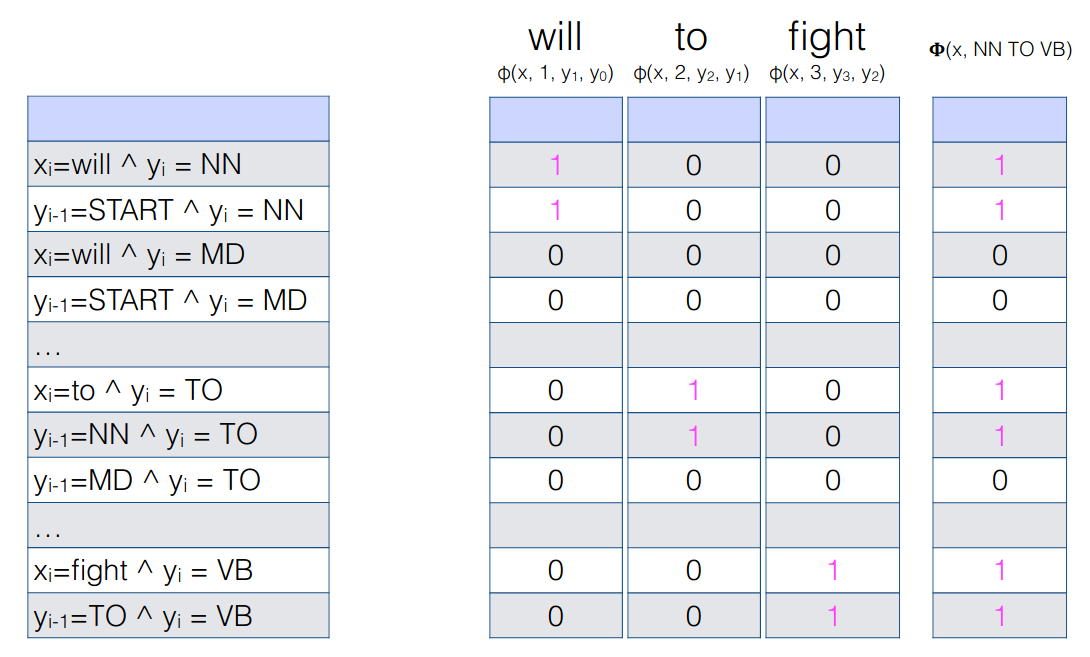
\includegraphics[scale=0.26]{pics/CRF3.png}
\caption{CRF Example}
\end{figure}
\footnotemark{Fuente: \url{http://people.ischool.berkeley.edu/~dbamman/nlpF18/slides/12_neural_sequence_labeling.pdf}}


\begin{itemize}

\item Suponemos que, para cualquier dimensión de $\vec{\Phi}_{[k]}, k= 1, \dots, d$, el $k$-ésimo atributo global es:

\begin{displaymath}
\vec{\Phi}(x_{1:m},s_{1:m})_{[k]} = \sum_{j=1}^{m} \vec{\phi}(x_{1:m},j,s_{j-1},s_j)_{[k]}
\end{displaymath}

\item Por lo tanto, $\vec{\Phi}(x_{1:m},s_{1:m})_{[k]}$ se calcula sumando el vector de características "local" $\vec{\phi}(x_{1:m},j,s_{j-1},s_j)_{[k]}$ sobre las $m$ transiciones de etiquetas diferentes en $s_1,\dots,s_m$.

\item Esperaríamos que cada vector local codifique información relevante sobre la transición de etiquetas activando algunas dimensiones del vector (estableciendo el valor en uno).

\item Ahora pasamos a dos problemas prácticos críticos en los CRFs: primero, la decodificación, y segundo, la estimación de parámetros (entrenamiento).

\end{itemize}



\section{Decodificación con CRFs}

\begin{itemize}

\item El problema de decodificación en los CRFs es el siguiente.
\item Dada una secuencia de entrada $x_{1:m} = x_1, x_2, \dots, x_m$, nos gustaría encontrar la secuencia de estados subyacente más probable bajo el modelo, es decir,

\begin{equation}
\begin{split}
\operatorname{arg} \max_{s_{1:m} \in S^m} P(s_{1:m}| x_{1:m}; \vec{w}) & = \operatorname{arg} \max_{s_{1:m} \in S^m} \frac{\exp (\vec{w} \cdot \vec{\Phi}(x_{1:m},s_{1:m}))}{\sum_{s'_{1:m} \in S^m}\exp (\vec{w} \cdot \vec{\Phi}(x_{1:m},s'_{1:m}))} \\
& = \operatorname{arg} \max_{s_{1:m} \in S^m} \exp (\vec{w} \cdot \vec{\Phi}(x_{1:m},s_{1:m})) \\
& = \operatorname{arg} \max_{s_{1:m} \in S^m} \vec{w} \cdot \vec{\Phi}(x_{1:m},s_{1:m}) \\
& = \operatorname{arg} \max_{s_{1:m} \in S^m} \vec{w} \cdot \sum_{j=1}^{m} \vec{\phi}(x_{1:m},j,s_{j-1},s_j) \\
& = \operatorname{arg} \max_{s_{1:m} \in S^m} \sum_{j=1}^{m} \vec{w} \cdot \vec{\phi}(x_{1:m},j,s_{j-1},s_j)
\end{split}
\end{equation}

\item Hemos demostrado que encontrar la secuencia más probable bajo el modelo es equivalente a encontrar la secuencia que maximiza:

\begin{displaymath}
\operatorname{arg} \max_{s_{1:m} \in S^m} \sum_{j=1}^{m} \vec{w} \cdot \vec{\phi}(x_{1:m},j,s_{j-1},s_j)
\end{displaymath}

\item Este problema tiene una intuición clara. Cada transición de la etiqueta $s_{j-1}$ a la etiqueta $s_j$ tiene un puntaje asociado: $\vec{w} \cdot \vec{\phi}(x_{1:m},j,s_{j-1},s_j)$.

\item Este puntaje podría ser positivo o negativo.

\item Intuitivamente, este puntaje será relativamente alto si la transición de estados es plausible, relativamente bajo si esta transición es implausible.

\item El problema de decodificación consiste en encontrar una secuencia completa de estados tal que la suma de los puntajes de transición sea maximizada.

\item Podemos resolver este problema utilizando una variante del algoritmo de Viterbi, de manera muy similar al algoritmo de decodificación para HMM o MEMM.

\end{itemize}


\section{Estimación de Parámetros en CRFs (Entrenamiento)}

\begin{itemize}

\item Para la estimación de parámetros, asumimos que tenemos un conjunto de $n$ ejemplos etiquetados, $\{(x_{1:m}^i, s_{1:m}^i )\}_{i=1}^n$. Cada $x_{1:m}^i$ es una secuencia de entrada $x_1^i, \dots , x_m^i$ y cada $s_{1:m}^i$ es una secuencia de etiquetas $s_1^i, \dots , s_m^i$.

\item Nuevamente, establecemos la log-verosimilitud negativa (o entropía cruzada) como la función de pérdida $L$ y optimizamos los parámetros utilizando el descenso de gradiente.

\item El principal desafío aquí es que los cálculos del gradiente $\frac{\partial L}{\partial \vec{w}_{[k]}}$ implican una suma sobre $S^m$ (un conjunto muy grande que contiene todas las posibles secuencias de etiquetas).

\item Esta suma se puede calcular de manera eficiente utilizando el algoritmo de avance-atrás (Forward-backward algorithm)\footnote{\url{http://www.cs.columbia.edu/~mcollins/fb.pdf}}.

\item Este es otro algoritmo de programación dinámica que está estrechamente relacionado con el algoritmo de Viterbi.

\end{itemize}


\section{CRFs y MEMMs}

\begin{itemize}

\item Los CRFs y los MEMMs son modelos de etiquetado de secuencias discriminatorios: modelan la probabilidad condicional directamente a través de una función lineal-logarítmica multiclase parametrizada (softmax).

\item Los HMM, por otro lado, son modelos generativos.

\item En los MEMM, la normalización (denominador del softmax) es local: ocurre en cada paso de la etiqueta (la suma se realiza sobre todos los valores de etiqueta posibles $S$).

\item En los CRFs, la normalización es global: la suma se realiza sobre todas las posibles secuencias de etiquetas $S^m$.

\item Entrenar un MEMM es bastante fácil: simplemente se entrena un modelo log-lineal multiclase para una palabra dada a la etiqueta. Este clasificador se utiliza en cada paso de la palabra para predecir toda la secuencia.

\item Entrenar un CRF es más complejo. El objetivo es maximizar la log-probabilidad de la secuencia más probable.

\end{itemize}



\subsection{CRFs y MEMMs: el problema del sesgo de etiqueta}

\begin{itemize}

\item Los MEMMs terminan tomando decisiones en cada paso de manera independiente.

\item Esto lleva a un problema llamado "sesgo de etiqueta": en algunas configuraciones del espacio de etiquetas, los MEMMs esencialmente ignoran aspectos importantes del contexto.

\item Ejemplo: La etiqueta correcta del POS para la oración "will to fight" (voluntad de luchar) es "NN TO VB" \footnote{Aquí estamos utilizando el conjunto de etiquetas PENN Treebank: \url{https://www.eecis.udel.edu/~vijay/cis889/ie/pos-set.pdf}}.

\item Aquí, NN significa "sustantivo", TO significa "infinitivo a" y VB significa "forma base verbal".

\item Los modales (MD) aparecen con mucha más frecuencia al comienzo de la oración que los sustantivos (por ejemplo, en preguntas).

\item Por lo tanto, la etiqueta "MD" recibirá un puntaje más alto que la etiqueta "NN" cuando $x_0$=``will'' : $P(s_1 = MD|s_{0} = *,x_1 = \text{``will''},...) > P( s_1 = NN| s_{i-1} = *, x_1 = \text{``will''})$.

\item Pero sabemos que MD + TO es muy raro: "puede comer", "quisiera comer".

\item La palabra "to" es relativamente determinística (casi siempre tiene la etiqueta TO), por lo que no importa qué etiqueta la preceda.

\item Debido a la normalización local de los MEMMs,  $P(s_i = TO | s_{i-1}, x_1, \dots, x_i = \text{``to''}, \dots, x_n)$ siempre será 1 cuando $x_i=$ "to", independientemente del valor de $s_{i-1}$ (MD o NN).

\item Eso significa que nuestra predicción para "to" no puede ayudarnos a desambiguar "will".

\item Perdemos la información de que las secuencias MD + TO rara vez ocurren.

\item Como consecuencia, es probable que un MEMM etiquete la primera palabra como "MD".

\item Los CRFs superan este problema al realizar una normalización global: consideran el puntaje de toda la secuencia antes de normalizarlo y convertirlo en una distribución de probabilidades.

\end{itemize}


\section{Enlaces}

\begin{itemize}

\item \url{http://people.ischool.berkeley.edu/~dbamman/nlpF18/slides/11_memm_crf.pdf}

\item \url{http://people.ischool.berkeley.edu/~dbamman/nlpF18/slides/12_neural_sequence_labeling.pdf}

\item \url{https://www.depends-on-the-definition.com/sequence-tagging-lstm-crf/}

\item \url{https://www.quora.com/What-are-the-pros-and-cons-of-these-three-sequence-models-MaxEnt-Markov-Model-Conditional-random-fields-and-recurrent-neural-networks}

\item \url{https://people.cs.umass.edu/~mccallum/papers/crf-tutorial.pdf}

\item \url{http://www.davidsbatista.net/blog/2017/11/13/Conditional_Random_Fields}

\end{itemize}


